\documentclass[11pt]{article}
%\usepackage{amsfonts}
\usepackage{amsmath}
\usepackage{fancybox}%,times}
\usepackage{graphicx,psfrag,epsf}
%\usepackage{amsmath}
\usepackage{enumerate}
\usepackage{graphicx,psfrag}
\usepackage{multirow}
\usepackage{epsfig}
%\usepackage{rotating}
\usepackage{subfigure}
\usepackage{theorem}
\usepackage{natbib,psfrag}
\usepackage{tikz}
\usepackage{xcolor}
\usepackage{kotex}
\newcommand{\blind}{0}
\usepackage{graphicx}
\DeclareGraphicsExtensions{.pdf,.png,.jpg}

\addtolength{\oddsidemargin}{-.75in}%
\addtolength{\evensidemargin}{-.75in}%
\addtolength{\textwidth}{1.5in}%
\addtolength{\textheight}{1.3in}%
%\addtolength{\topmargin}{-.6in}%
\addtolength{\topmargin}{-.8in}%

%\theoremstyle{break}
\newtheorem{The}{Theorem}
\newtheorem{Def}{Definition}
\newtheorem{Pro}{Proposition}
\newtheorem{Lem}{Lemma}
\newtheorem{Cor}{Corollary}
\newtheorem{asp}{Assumption}


\renewcommand{\thefootnote}{\arabic{footnote}}
%\renewcommand{\thefootnote}{\alph{footnote}}
%\renewcommand{\thefootnote}{\roman{footnote}}
%\renewcommand{\thefootnote}{\fnsymbol{footnote}}

\begin{document}
	
	
	%\bibliographystyle{natbib}
	
	\newcommand{\Ito}{$It\hat{o}$'$s~Lemma$}
	
	\newcommand\ind{\stackrel{\rm ind}{\sim}}
	\newcommand\iid{\stackrel{\rm iid}{\sim}}
	\renewcommand\c{\mathbf{c}}
	\newcommand\y{\mathbf{y}}
	\newcommand\z{\mathbf{z}}
	\renewcommand\P{\mathbf{P}}
	\newcommand\W{\mathbf{W}}
	\newcommand\X{\mathbf{X}}
	\newcommand\Y{\mathbf{Y}}
	\newcommand\Z{\mathbf{Z}}
	\newcommand\J{{\cal J}}
	\newcommand\B{{\cal B}}
	\newcommand\K{{\cal K}}
	\newcommand\N{{\rm N}}
	\newcommand\bs{\boldsymbol}
	\newcommand\bth{\bs\theta}
	\newcommand\bbe{\bs\beta}
	\renewcommand\*{^\star}
	
	\def\spacingset#1{\renewcommand{\baselinestretch}%
		{#1}\small\normalsize} \spacingset{1}
	
	
	%%%%%%%%%%%%%%%%%%%%%%%%%%%%%%%%%%%%%%%%%%%%%%%%%%%%%%%%%%%%%%%%%%%%%%%%%%%%%%
	
	\bigskip
	\bigskip
	\bigskip
	\begin{center}
		{\LARGE\bf September 05, 2019 }
	\end{center}
	\medskip
	
	%\begin{abstract}
	%\end{abstract}
	
	%\noindent%
	%{\it Key Words:}  AECM algorithm; Astrophysical data analysis;
	%ECME algorithm; Incompatible Gibbs sampler; Marginal data
	%augmentation; Multiple imputation; Spectral analysis
	
	\spacingset{1.45}
	
	
	
	
	
	\section{Regression Spline}
	
	Assume that the range of x is $[a,b]$. Let the point
	$$ a < \xi_1 < \dots < \xi_K < b$$
	be a partion of the interval $[a,b]$  
	$\left\{ \xi_1 , \dots , \xi_K \right\}$ are called knots.
	
	\subsection{Radial Basis Function}
	A RBF $\varphi$ is a real valued function whose value depends only on the distance from origin.
	A real function $\varphi : [0,\infty) \rightarrow {\rm I\!R}$ with a metric on space $\| \cdot \| : V \rightarrow [0,\infty)$ a function $\varphi_c = \varphi(\|\mathbf{x} - \mathbf{c}\|)$ is said to be a radial kernel centered at c. A radial function and the associated radial kernels are said to be radial basis function
	
	We use radial basis functions defined by
	$$
	\mathbf{b}(u) = \left\{  u, \left| \frac{u-\tau_1}{c} \right|^3 , \cdots , \left| \frac{u-\tau_K}{c} \right|^3 \right\}
	$$
	where $c$ is sample standard deviation 
	
	\section{Simulation}
	Let
	$$y = \sum_{l=1}^{4} f_l(X_l) + \sum_{k=1}^{4} Z_k \theta_k + e $$
	
	\begin{align*}
	f_1(x) &= 3exp(-30(x-0.3)^2)+exp(-50(x-0.7)^2)\\
	f_2(x) &= sin(2\pi x)\\
	f_3(x) &= x \\
	f_4(x) &= 0\\
	\theta_1 &= 0.6\\
	\theta_2 &= -1\\
	\theta_3&=\theta_4 = 0
	\end{align*}
	Make spline and centerize the data we can get $\tilde{y}$
	
	\begin{align*}
	\tilde{y} &= y -\bar{y} = b_1(X_1)\beta_1 + b_2(X_2)\beta_2 + b_3(X_3)\beta_3 + b_4(X_4)\beta_4 + \sum_{k=1}^{4} Z_k \theta_k + e
	\end{align*}
	
	
	\subsection{MFVB method}
	
	Setting prior as
	\begin{align*}
	Y|\tau,\beta  &\sim N(X\beta , \sigma^2 \cdot I_N)\\
	\beta_i | \gamma_i &\sim^{ind} N(0,\sigma_{\beta}^2) \text{ for } i=1,\dots p \\
	\sigma_{\beta}^2 &\sim Inverse-Gamma(a,b) \\
	\sigma^2 &\sim Gamma(c,d)   
	\end{align*}
	
	
	
	By Baye's rule
	$$
	p(\tau,\gamma ,\beta | Y) \propto p(Y|\tau,\beta) p(\beta | \gamma) p(\tau) p(\gamma) 
	$$
	Then variational distribution is
	$$
	p(\tau,\gamma ,\mu | Y) \approx q(\tau,\gamma,\mu) = q_1(\tau) q_2(\gamma) q_3(\mu)
	$$
	we can maximize ELBO by coordinate descent algorithm
	
	\begin{align*}
	q_1^*(\sigma^2) &= E_{q_2,q_3}[p(\sigma^2,\gamma ,\beta | Y)] \propto E_{q_2,q_3}[p(Y|\sigma^2,\beta)  p(\tau)]\\
	q_2^*(\sigma_{\beta}^2) &= E_{q_1,q_3}[p(\tau,\sigma_{\beta}^2 ,\beta | Y)] \propto E_{q_1,q_3}[ p(\beta | \sigma_{\beta}^2)   p(\sigma_{\beta}^2)]\\
	q_3^*(\beta) &= E_{q_1,q_2}[p(\tau,\gamma ,\beta | Y)] \propto E_{q_1,q_2}[p(Y|\tau,\beta) p(\beta | \gamma)   ]\\
	\end{align*}
	
	Then
	
	\begin{align*}
	q_1^* &\sim Gamma\left(c + \frac{N+1}{2}, d + \frac{1}{2}\left\{Y'Y -E_{q3}[\beta'](X'Y)\right\} + tr\left[X(var_{q3}[\beta]+E_{q3}[\beta]E_{q3}[\beta'])X'\right]\right)\\
	q_2^* &\sim \prod_{i=1}^{p}Inverse-Gamma( a+ \frac{1}{2}, b + \frac{1}{2}\{var_{q3}[\beta]_{i,i} +E_{q3}[\beta_i]^2 \})\\
	q_3^* &\sim N\left(E_{q1}[\sigma^2]\Sigma X'Y,\left(diag(E_{q2}[\sigma_{\beta}^2]) + E_{q1}[\sigma^2]X'X \right)^{-1} = \Sigma \right)
	\end{align*}
	

	
	\subsection{MFVB method with variable selection}
	
	Variable selection model is
	
	\begin{align*}
	Y = X\Gamma\beta + \epsilon , \;\;\; \epsilon \sim N(0,\sigma^2 I)
	\end{align*}
	
	where 
	
	\begin{align*}
	Y|\beta,\sigma^2 ,\gamma &\sim N(X\Gamma\beta , \sigma^2 I)\\
	\sigma^2 &\sim Inverse-Gamma(A,B)  \;\;\;\ A=0,\;B=0\\
	\beta_j &\sim N(0, \sigma_{\beta}^2)\\
	\gamma_j &\sim Bernoulli(\rho) \;\;\;\ \rho=0.5
	\end{align*}
	


	
	
	\subsection{MFVB method with variable selection hierarchical model}
	
	Variable selection hierarchical model is
	
	\begin{align*}
	Y = X\Gamma\beta + \epsilon , \;\;\; \epsilon \sim N(0,\sigma^2 I)
	\end{align*}
	
	where 
	
	\begin{align*}
	Y|\beta,\sigma^2 ,\gamma &\sim N(Z\Gamma\beta , \sigma^2 I)\\
	\sigma^2 &\sim Inverse-Gamma(A,B)  \;\;\;\ A=0,\;B=0\\
	\beta_j &\sim N(0, \sigma_{\beta}^2)\\
	\gamma_j &\sim Bernoulli(\rho)\\
	\rho &\sim Beta(C,D) \;\;\;\ C=1,\;D=1.4
	\end{align*}
	
	
	\begin{align*}
	p(\beta,\sigma^2,\sigma_\beta^2,\Gamma | Y) \approx q(\beta,\sigma^2,\sigma_\beta^2,\Gamma) = \prod_{j=1}^{p}q_1^*(\beta_j)q_2^*(\sigma^2) q_3^*(\rho)\prod_{j=1}^{p}q_4^*(\gamma_j)
	\end{align*}
	Use coordinate ascent algorithm, $q$ density of $\beta$ is
	\begin{align*}
	q_1^*(\beta) &\propto E_{-q_1}\left[p(\beta,\sigma^2,\sigma_\beta^2,\Gamma , \rho,Y)\right]\\
	&\propto E_{-q_1}\left[\exp\left(-\frac{1}{2\sigma^2}\left(Y - Z\Gamma\beta\right)'\left(Y-Z\Gamma\beta\right) - \frac{1}{2}\sum_{j=1}^{p}\frac{\beta_j^2}{\sigma_{\beta}^2}\right)\right]\\
	&\propto \exp\left(-\frac{1}{2} \beta'\left<D\right> -\frac{1}{2}\left<\frac{1}{\sigma^2}\right>\left(\beta'\left<\Gamma\right>'Z'Z\left<\Gamma\right>\beta- 2\beta'\left<\Gamma\right>'Z'Y\right)\right)\\
	&\propto \exp\left(-\frac{1}{2}\left[\beta'\left(\left<D\right> + \left<\frac{1}{\sigma^2}\right>\left<\Gamma\right>'Z'Z\left<\Gamma\right>\right)\beta -2 \left<\frac{1}{\sigma^2}\right>\beta'\left<\Gamma\right>'Z'Y\right]\right)\\
	&\sim N(\mu,\Sigma)
	\end{align*}
	Where $D = diag(\frac{1}{\sigma_{\beta}^2})$ , $<>$ means expectation under $q$ functions and
	\begin{align*}
	\Sigma = \left(\left<D\right> +\beta' \left<\frac{1}{\sigma^2}\right>\left<\Gamma\right>'Z'Z\left<\Gamma\right>\right)^{-1},\;\;\;\mu = \left<\frac{1}{\sigma^2}\right> \Sigma  \left<\Gamma\right>'Z'Y
	\end{align*}
	$q$ density of $\sigma^2$ is
	\begin{align*}
	q_2^*(\sigma^2) &\propto E_{-q_2}\left[p(\beta,\sigma^2,\sigma_\beta^2,\Gamma, \rho , Y)\right]\\
	&\propto E_{-q_2}\left[\left(\sigma^2\right)^{-\left(\frac{n}{2}+a\right)-1}\exp \left(-\frac{1}{\sigma^2}\left(b+\left(Y-Z\Gamma\beta\right)'\left(Y-Z\Gamma\beta\right)\right)\right) \right]\\
	&\propto Inverse-Gamma\left(a+\frac{n}{2}, b+\frac{1}{2}\left(Y'Y - 2\left<\beta\right>'\left<\Gamma\right>'Z'Y + tr\left(\left(Z'Z \odot \Omega\right)\left(\mu \mu'+ \Sigma\right)\right) \right)\right)
	\end{align*}
	Where $\odot$ is hadamard product and
	\begin{itemize}
		\item $\gamma = (\gamma_1,\dots,\gamma_p)$
		\item $\Omega = \left<\gamma\right>\left<\gamma\right>' + \left<\Gamma\right>\odot(I - \left<\Gamma\right>)$
	\end{itemize}
	$q$ density of $\rho$ is
	\begin{align*}
	q_3^*(\rho) &\propto E_{-q_3}\left[p(\beta,\sigma^2,\sigma_\beta^2,\Gamma, \rho , Y)\right]\\
	&\propto \rho^{C-1} \left(1-\rho\right)^{D-1} \prod_{j=1}^{p} \rho^{\gamma_j} \left(1-\rho\right)^{1-\gamma_j}\\
	&\propto \rho^{C+\sum_{j=1}^{p}\gamma_j-1} \left(1-\rho\right)^{D+p -\sum_{j=1}^{p}\gamma_j -1}\\
	&\sim Beta(C+\sum_{j=1}^{p}\gamma_j, D+p -\sum_{j=1}^{p}\gamma_j)
	\end{align*}
	$q$ density of $\gamma$ is
	\begin{align*}
	q_4^*(\gamma) &E_{-q_4}\left[\propto \prod_{j=1}^{p} \rho^{\gamma_j}(1-\rho)^{-\gamma_j} \exp(-\frac{1}{2}\frac{1}{\sigma^2}\left(\beta'\Gamma'Z'Z\Gamma\beta - 2\beta'\Gamma'Z'y\right))\right]\\
	&\propto\exp\left[ \gamma_j \left( \left<\log\left(\rho/(1-\rho)\right)\right> -\frac{1}{2}\left<\frac{1}{\sigma^2}\right> \left<\beta_j^2\right> Z_j'Z_j + \left<\frac{1}{\sigma^2}\right> Z_j'\left[Y\mu_j - X_{-j}\left<\Gamma_{-j}\right>\left(\mu_{-j}\mu_j + \Sigma_{-j,j}\right)\right] \right)\right]
	\end{align*} 
	Where
	\begin{itemize}
		\item $X_j$ means $j$th coloumn of $X$
		\item $X_{-j}$ means without $j$th column
		\item $X_{-i,j}$ means $j$th column without $i$th component 
		\item $\mu_j$ is $j$th component of vector and $mu_j$ means without $j$th component
	\end{itemize}
	
	\begin{figure}
		\centering
		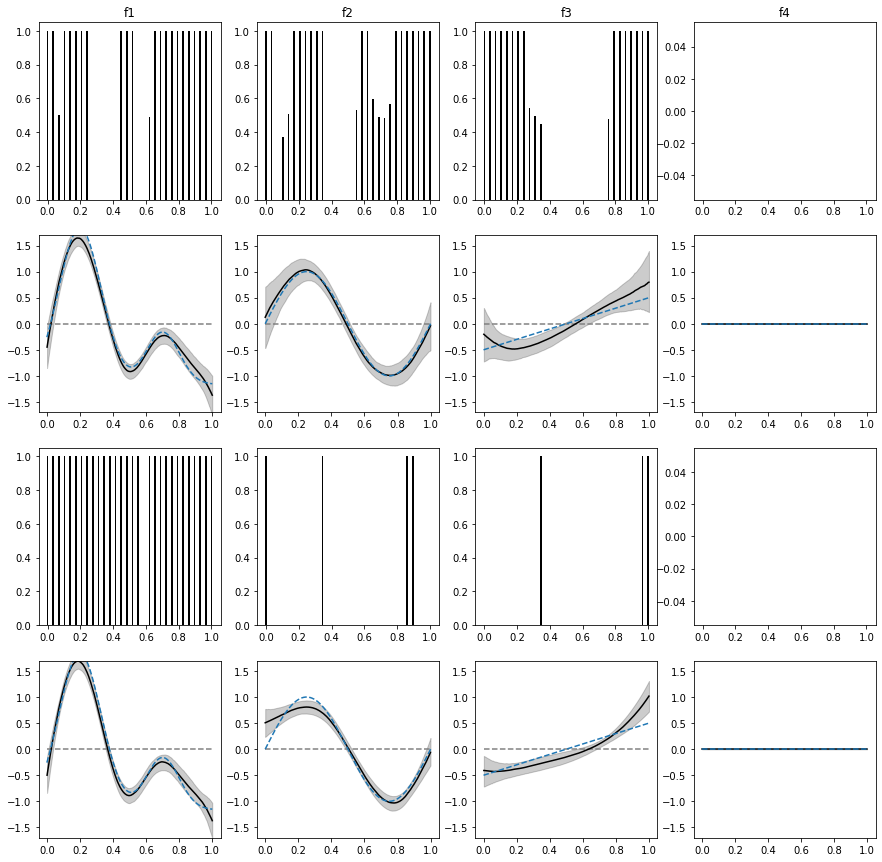
\includegraphics[width=1\linewidth]{plot1}
		\caption{Compare the variable selection model without Beta prior and without Beta prior. First and Second row has plat prior $\rho = 0.5$. Third and Forth row has beta prior $\rho \sim Beta(1,1.4)$}
		\label{fig:plot1}
	\end{figure}
	
	\subsubsection{Posterior of $rho$}
	
	\begin{align*}
		f_1(x) &= 3exp(-30(x-0.3)^2)+exp(-50(x-0.7)^2)\\
	f_2(x) &= sin(2\pi x)\\
	f_3(x) &= x \\
	f_4(x) &= 0\\
	\end{align*}

\begin{tabular}{|c|c|c|c|c|c|}
	\hline 
	$\rho\sim$ & $Beta(1, 1.4)$ & $Beta(1, 1)$ & $Beta(1, 2)$ & $Beta(2, 1)$ &  $Beta(2, 2)$\\ 
	\hline 
	f1 $q^*(\rho) \sim$&beta(30.0 2.4)  &beta(31.0 1.0)  &beta(4.0, 29.0)  & beta(32.0 1.0) & beta(22.8,10.2) \\ 
	\hline 
	f2 $q^*(\rho) \sim$& beta(5.0 27.4) & beta(31.0 1.0) &beta(3.0, 30.0)  & beta(32.0 1.0) & beta(26.9 6.1) \\ 
	\hline 
	f3 $q^*(\rho) \sim$& beta( 4.0, 28.4) & beta(31.0 1.0) & beta(4.0, 30.0) & beta(32.0 1.0) & beta(26.9 6.1) \\ 
	\hline 
	f4 $q^*(\rho) \sim$& beta(1.0 31.4) & beta(1.0 31.0) & beta(1.0 32.0) &beta(32.0 1.0)  & beta(30.0 3.0) \\ 
	\hline 
\end{tabular} 

	

	
\end{document}